\section{Introduction}\label{sec:introductio}
Linux, which was introduced in 1991, is the most commonly deployed operating system in the market~\cite{Love2010}. Even though it has many different distributions, they all share the same kernel module and interface~\cite{Bovet2006}. A key component of the kernel is the Virtual Filesystem (VFS)~\cite{Sandberg1988}, which implements the file and filesystem-related interfaces provided to user-space programs. This allows programs to use standard Unix system calls to read and write to various filesystems, even on different media or across the network. This allowed for the creation of many local and distributed filesystems, including Sun Microsystems' NFS~\cite{Sandberg1988} and Google's GFS~\cite{Ghemawat2003}, as well as many device drivers, like character device drivers~\cite{Salzman2009, Corbet2005}.

When software system developers need to learn about the Linux kernel APIs, they face a difficulty learning about it from the documentation. This is because the documentation usually lacks sufficient examples and explanations. The widespread nature of this issue~\cite{Lethbridge2003, Robillard2009} has lead developers to use other forms of documentation, like wikis, blogs, and online question and answer communities like Stack Overflow, where people ask questions and others answer them.
The problem of documentation is especially prevalent for the filesystem APIs, because it contains many functions which seem to share the same goal, as well as many flags and arguments which can completely alter the behavior of the function~\cite{Love2010}.

Recently, many studies have shown that the POSIX standard API, which the Linux kernel filesystem APIs follow, have many drawbacks for modern operating systems. Zadok et al~\cite{Zadok2017} highlight some of the issues in POSIX and propose some ideas to improve it or replace it. One major issue they mention is that, by design, POSIX interface methods are susceptible to ``Time of Check To Time of Use'' (TOCTTOU) vulnerabilities~\cite{Wei2005}. Additionally Atlidakis el al~\cite{Atlidakis2016} explain how the common applications have designed around the POSIX APIs to overcome their shortcomings, and how this practice is not sustainable and can lead to suboptimal performance.

This study highlights how one the Linux kernel filesystem, which follow POSIX standards, are asked about on Stack Overflow. This aims to understand the software engineering viewpoint on the filesystem APIs and whether developers discuss the design issues mentioned above on Stack Overflow. More generally, it aims to understand what questions are asked about these APIs on Stack Overflow. We do that by extracting single-word, bigram and trigram frequencies in questions that contain at least one of the filesystem APIs. We also examine which filesystem APIs are likely to be asked about together, indicating codependency or confusion.

The contributions of this study are as follows:
\begin{itemize}
  \item We demonstrate that Stack Overflow is a somewhat reliable source of information on Linux filesystem APIs.
  \item We show that the community is still engaged in questions and discussions about Linux filesystem APIs, even after about 30 years from its birth.
  \item We quantitatively study which keywords are the most common in questions are asked about the APIs.
  \item We examine which filesystem APIs are likely to be asked about together, indicating codependency or confusion.
\end{itemize}

\section{Related Work}\label{sec:relatedw}

Some studies try to use Stack Overflow to give suggestions on usage and code examples inside an ide~\cite{Ponzanelli2014}. There is even a python module that loads examples from Stack Overflow as modules in the code\footnote{https://github.com/drathier/stack-overflow-import}
Other studies on Stack Overflow have looked qualitatively and quantitatively into Unanswered questions~\cite{Asaduzzaman2013} to understand why they are still unanswered, and on Deleted questions~\cite{Correa2014} to understand the reasons behind the deletion. Gruetze et al.~\cite{Gruetze2016} study the dynamics and topic shifts of Stack Overflow over time. Vasilescu et al~\cite{Vasilescu2013} study how the activity of users on Github affects their activity on Stack Overflow.

The closest study to ours is the early investigation into the coverage and dynamics of crowd documentation on Stack Overflow by Parnin et al.~\cite{Parnin2012CrowdDE}, where they studied several Java APIs and how much of the classes had questions asked about them on Stack Overflow. Another close study is by Kavaler et al.~\cite{Kavaler2013}, which discusses the relationship between usage of an Adnroid API mined from real application to the questions asked about it on Stack Overflow. The first half of our study discusses similar research questions but in a different language (C instead of Java), with different demographics, and a relatively older API.

\section{Methodology}\label{sec:methodology}
In this section, we explain our research questions, how we collected our data, and how we analyzed it.
\subsection{Research Questions}\label{subsec:rq}
First, it is important to study whether we can rely on the Stack Overflow community as a documentation of Linux kernel filesystem APIs, and whether we can rely on it to study questions related to that API. To achieve that, we first examine the coverage of the filesystem API on Stack Overflow. Coverage in our context refers to the percentage of filesystem functions and structures for which there are at least $n$ questions that mention it on Stack Overflow. We also examine the relationship between the usage of a function in opensource projects on GitHub and the amount of questions that mention it. Since the API is old, we wanted to see whether it is still discussed in Q\&A communities, and where these discussions are going. Additionally, this part of the study if the results and the general trends identified in previous studies~\cite{Parnin2012CrowdDE} also apply to our dataset.
Second, we need to understand what kinds of problems are Stack Overflow users face when dealing with the filesystem API, which could influence future designers of the APIs. Therefore, we ask about the types of questions asked about the filesystem APIs. Since such question is broad, we focus on the most common keywords in questions and how often do functions appear together in the same function.

We study the following questions:
\begin{itemize}
  \item
  \textbf{RQ1} Can we rely on the Stack Overflow crowd to discuss all of Linux kernel filesystem APIs?
  \begin{itemize}
    \item
    \textbf{RQ1.1} Are the API methods widely covered?
    \item
    \textbf{RQ1.2} Is there a relationship between number of discussions around a function and its usage in Github repositories?
    \item
    \textbf{RQ1.3} Are there still ongoing discussions about these APIs? How fast are they covered?
  \end{itemize}
  \item
  \textbf{RQ2} What kind of questions are asked about the APIs?
  \begin{itemize}
    \item
    \textbf{RQ2.1} What are the most common keywords that appear in questions?
    \item
    \textbf{RQ2.2} How often do pairs of components appear together in questions?
  \end{itemize}
  \item
\end{itemize}

\subsection{Data Collection}\label{subsec:data}
\subsubsection{Filesystem API}
To extract the filesystem API, we used a script to scrape function and structure names, along with the categories they fall into from the official Linux kernel v4.16.0 documentation\footnote{https://www.kernel.org/doc/html/v4.16/filesystems/index.html}, then we manually verified them. The latest documentation is well-formatted, so it was easy to extract header names and using a script written in jquery. The result was loaded to a database, where each function was given a unique id and assigned to a category. In total, we extracted 310 functions and structures, classified into 14 different categories.

\subsubsection{Stack Overflow}
Stack Exchange, the company behind Stack Overflow and other Q\&A websites, publishes data dumps of the databases of all its websites, under a Creative Commons license on archive.org\footnote{https://archive.org/details/stackexchange} once every three months. We downloaded a database dump of Stack Overflow that dates to 12/2017, converted the XML to SQL and loaded on a relational database using a tool called SODDI\footnote{https://github.com/BrentOzarULTD/soddi}. Due to the huge size of data (42 Gb after loading to the database, for 39 million records), we only considered posts which contained the following tags: \textit{c, c++, linux, kernel, kernel-module, posix, and driver}. Since answers are not tagged, we included all the answers on matched questions. All stackoverflow posts are required to be tagged, and most tags are accurate since Stack Overflow is heavily moderated. The tags in the data dump are listed in plain text inside the posts table, and not in a separate table, so to improve the performance of the data filtering, the tags column was added to a fulltext index~\cite{Hamilton2001}. This resulted in an order of magnitude increase in performance over a regular expression search (several minutes instead of several hours) with a slight decrease in recall. The filtered dataset contains 3.1 million records and is 4.5 Gb in size.

\subsubsection{Linking Methodology}
To gather our data, we used a process adopted from Parnin et al.~\cite{Parnin2012CrowdDE}.
In our case, a link is a connection between a StackOverflow question and a filesystem API function or structure. Figure \ref{fig:soq} shows a sample Stack Overflow question annotated with the different types of links: word links which occur in regular text, code links occur in \texttt{<code></code>} tags and include a single function or class name, and code block links are enclosed within \texttt{<pre></pre>} tags representing examples and stack traces. We searched the title and body of the questions and related answers for any mentions of filesystem function and structures using case-insensitive word-boundary full text search, and recorded the results in the database. We found a total of 981 matches between posts and functions.

\begin{figure*}[t!]
  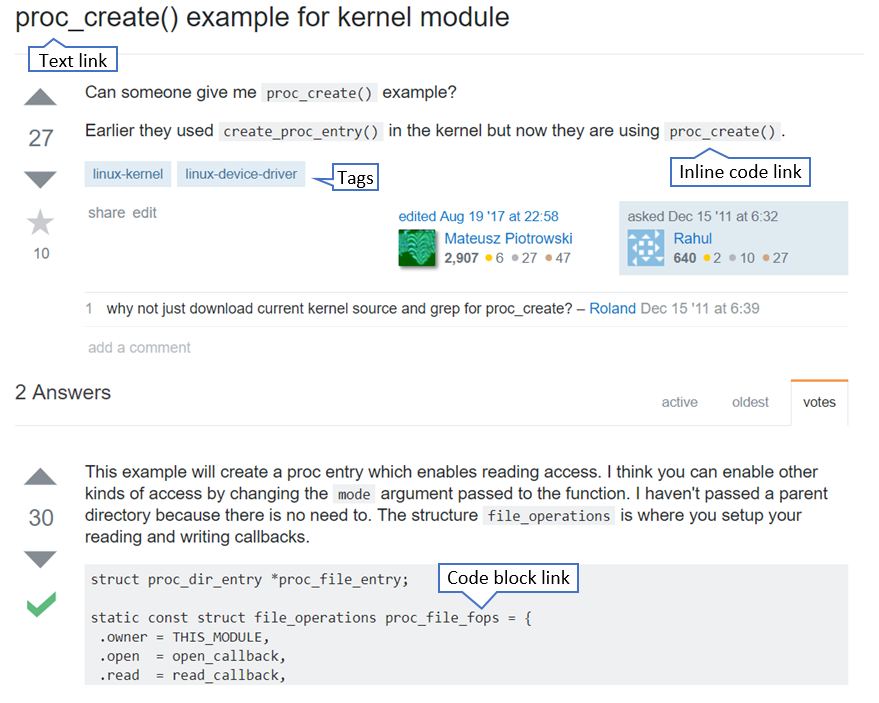
\includegraphics[width=0.75\textwidth]{images/soquestion-annotated.png}
  \caption{A sample Stack Overflow question with different types of links}
  \label{fig:soq}
\end{figure*}

\subsubsection{Usage Data}
The usage data was gathered by searching for the filesystem API functions on the Github code search API\footnote{https://developer.github.com/v3/search/\#search-code}. We used a script that issued one request for each function and recorded the total number of records reported by the response. We limited our search to files written in \texttt{C} only to prevent any similarly named functions from other programming languages from inflating the search result. Between each API call, we waited a random period of time between 3-10 seconds to comply with the rate limits and robot detection imposed by the server. We note that Github code search does not include forked repositories unless they have more stars than the original repositories.

\begin{figure*}[t!]
  \centering
  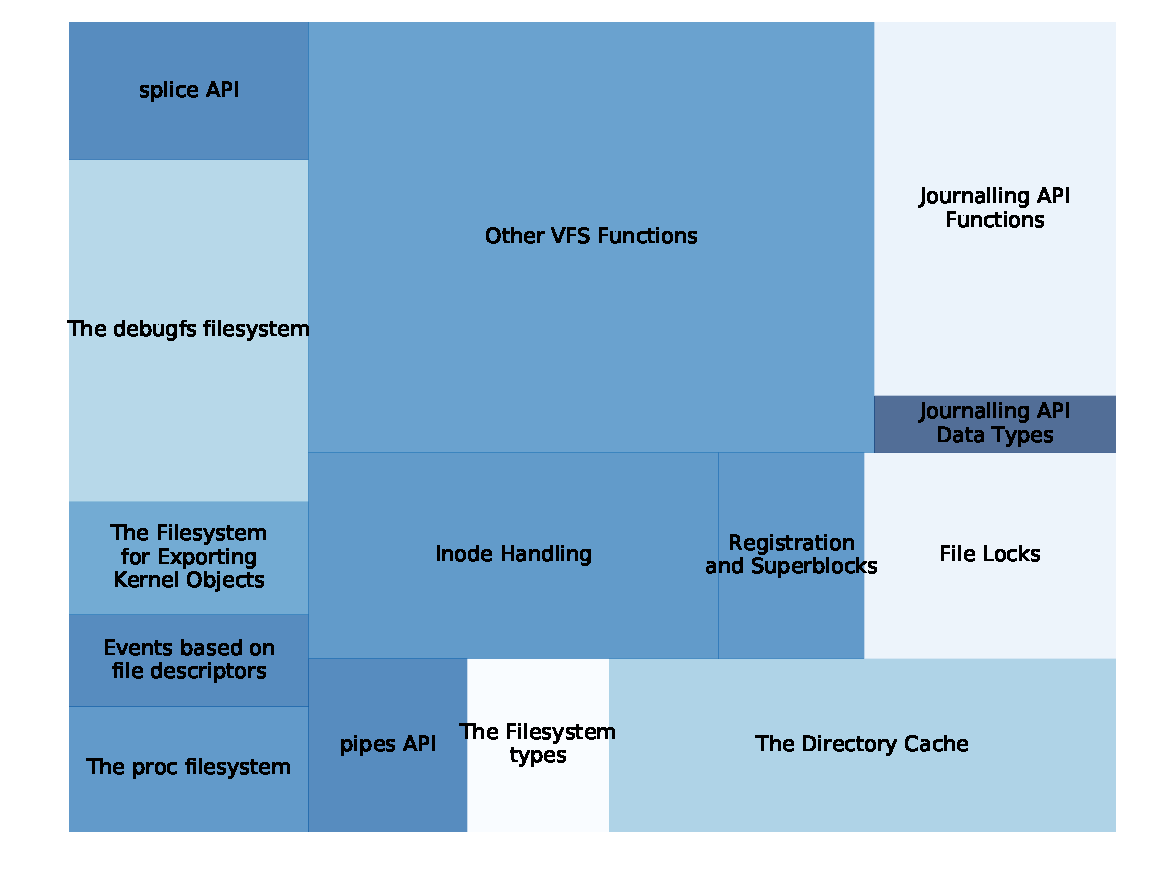
\includegraphics[width=0.7\textwidth]{scripts/figures/1-1-coveragebycategory.pdf}
  \caption{Coverage of Linux filesystem API by category, $n=1$. Darker colors indicate higher coverage, and the size of each cell represents the number of functions in that category}
  \label{fig:covbycategory}
\end{figure*}

\subsection{Data Analysis}\label{subsec:analysis}
Most research questions (all RQ1 and RQ2.2) are satisfied by queries on the cached list of results recorded on the database joined with the original question data. RQ2.1 includes a technique in natural language processing called frequency analysis, described below.

\subsubsection{Frequency Analysis}
To answer RQ2.1, we performed a basic frequency analysis with single words, bigrams and trigrams on the questions and their answers. First, we sanitized question texts by removing all html tags and code blocks since they are irrelevant to what the question asks. Then, we tokenized the texts by word boundary, and stemmed them using porter stemmer~\cite{Porter1980}. After that, we filtered out words we considered stop words, including the list of default stop words in the English language, combined with other stop words common in Stack Overflow conversations, such as "code", "please", "thanks". Finally, we generated single words, bigrams and trigrams, and fed each of them individually to a frequency counter. We applied this method for question titles and bodies without the answers, and then to the answers only.

\subsection{Reproducibility}\label{subsec:repr}
All our data is provided publically on GitHub. The following repository contains scripts, queries and result csv files used in this paper:

https://github.com/zalsader/LinuxFSQuestions

\section{Results and Discussion} \label{sec:results}
\subsection{Data Reliability}
In this subsection, we examine the results of our first research question: \textbf{RQ1 Can we rely on the Stack Overflow crowd to discuss all of Linux kernel filesystem APIs?}
\subsubsection{Extent of Coverage}
\textbf{RQ1.1 Are the API methods widely covered?}
To answer our first question, we considered the coverage of API functions and structures. We define coverage as the percentage of API elements that have at least $n$ questions discussing the function/structure, where $n$ is called the saturation level. We found that less than third (32.9\%) of the functions have at least on thread discussing them on Stack Overflow, while the percentage decreases considerably as $n$ increases. For $n=2$, 15.8\% of the functions are covered, and for $n=5$ and $10$, the coverage is 8.4 and 4.2 respectively. From this, we conclude that Stack Overflow is reliable to a moderate extent for filesystem APIs, which allows us to continue our analysis. The moderate coverage could be due to the small size of novice programmers interested in these APIs, which generates a smaller number of questions compared to other subjects like Android for example.

Additionally, we examined the coverage of API functions per category, as shown in Figure \ref{fig:covbycategory}. The coverages varied between 0\% to 60\%, with a median of 44\%. The figure shows that there are no big differences in coverage between most categories.

\subsubsection{Usage vs Discussion}
\textbf{RQ1.2 Is there a relationship between number of discussions around a function and its usage in Github repositories?}
To explain why many functions have no or little mention on Stack Overflow, we compare the number of references to each function from the previous step to the data we collected from GitHub. Results are plotted in Figure \ref{fig:usageref} on a log-log scale. We find that there is a moderately strong correlation between the log of usage of a function and the log of questions asked about it, with a slope of 0.51 and Pearson's regression coefficient of 0.65. This translates into a sublinear dependence of y on x, meaning that, on average, the demand for function documentation from Stack Overflow grows slower than the function usage in the code. This is consistent with past studies, and can be attributed to the fact that there is a finite amount of questions that could be asked about a function before all questions are asked on Stack Overflow. The average slope in our case is higher than the average slope in the related studies (0.31 in~\cite{Kavaler2013}), which can be explained because the average coverage is less than the projects considered by related studies.

\begin{figure}[t!]
  \centering
  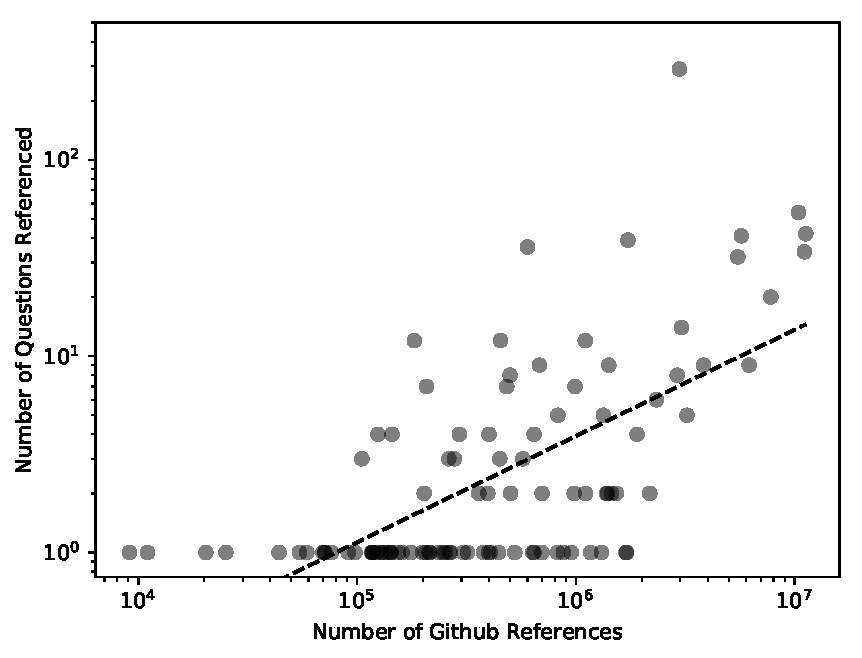
\includegraphics[width=\columnwidth]{scripts/figures/1-2-usage-vs-coverage.pdf}
  \caption{Usage vs number of references in Stack Overflow on a log-log scale. The dashed line represents the trend between the points}
  \label{fig:usageref}
\end{figure}

\subsubsection{Discussion over time}
\textbf{RQ1.3 Are there still ongoing discussions about these APIs? How fast are they covered?}
To answer this question, we examine the coverage with different values of $n$ over time. We notice that coverage is increasing slowly but steadily over time for $n=1$, while there was a relatively short period of stability for $n>2$ between 2016 and 2017. It is interesting to see that the coverage is still growing steadily even after around 30 years from creation of the API. This means that users are still facing new problems and asking new questions that no one asked about before on the website. This also indicates that even the newer versions of the documentation still have not kept up with the questions people ask about the filesystem APIs.

\begin{figure}[t!]
  \centering
  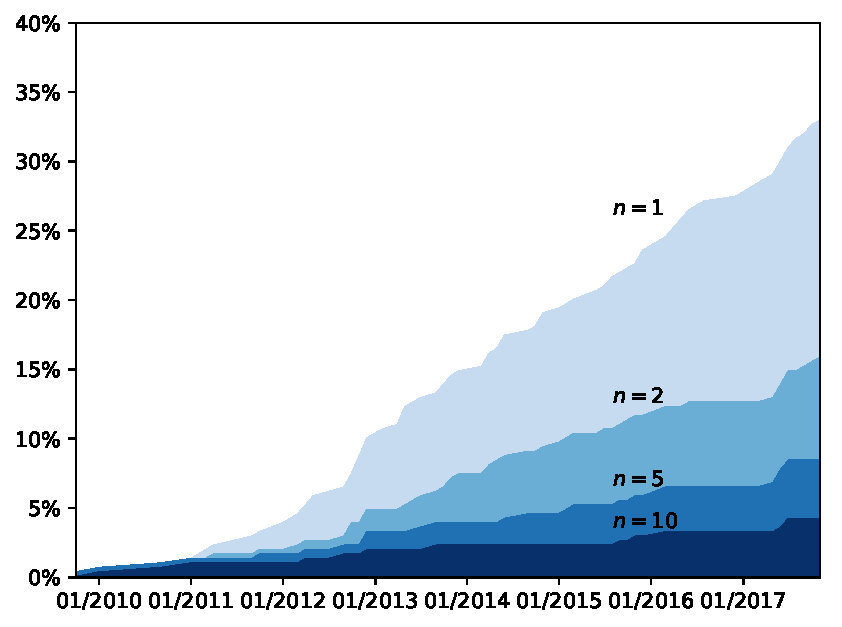
\includegraphics[width=\columnwidth]{scripts/figures/1-3-coverage-by-time}
  \caption{The coverage for the API over time}
  \label{fig:coveragetime}
\end{figure}

\subsection{Questions asked about the API}
In this subsection we examine and discuss the results from our second research question: \textbf{RQ2 What kind of questions are asked about the APIs?}
\subsubsection{Common Keywords}
\textbf{RQ2.1 What are the most common keywords that appear in questions?}
To answer this question, we identify the keywords that are most commonly found in questions and answers that contain any of the linux filesystem API functions and structures, excluding code samples as defined in Subsection~\ref{subsec:data}. Since the words are stemmed using the porter stemmer, many of the terms in the figure appear to be misspelled or incomplete.
From the single word results, it seems that most questions ask about how to `use' the functions, how they `work', and some also ask for `examples'. Since we are asking questions about the filesystem API, the words `write', `read' and `kernel' appeared very often. In addition, a lot of questions reported `problems' or asked for `solutions'. The results from mining answers for single word frequency do not seem very different.

The results for bigrams and trigrams seem to result in more interesting terms, after the most common `kernel module' and `linux kernel module', many questions contained `device driver', `block device' and `linux device driver' in reference to questions about vfs functions related to device drivers, like this post \footnote{https://stackoverflow.com/q/11578504}, which asks about ``how \texttt{sys\_open} works?'' in the context of a character device driver. Additionally, many questions asked for a `better way', or the `best way' to achieve a task. The results from mining bigrams and trigrams of answers are very similar, with the difference that `better way', `best way' and `create new' appear more often than other terms in the question.

\begin{figure*}[t!]
  \centering
  \subfloat[Single Words]{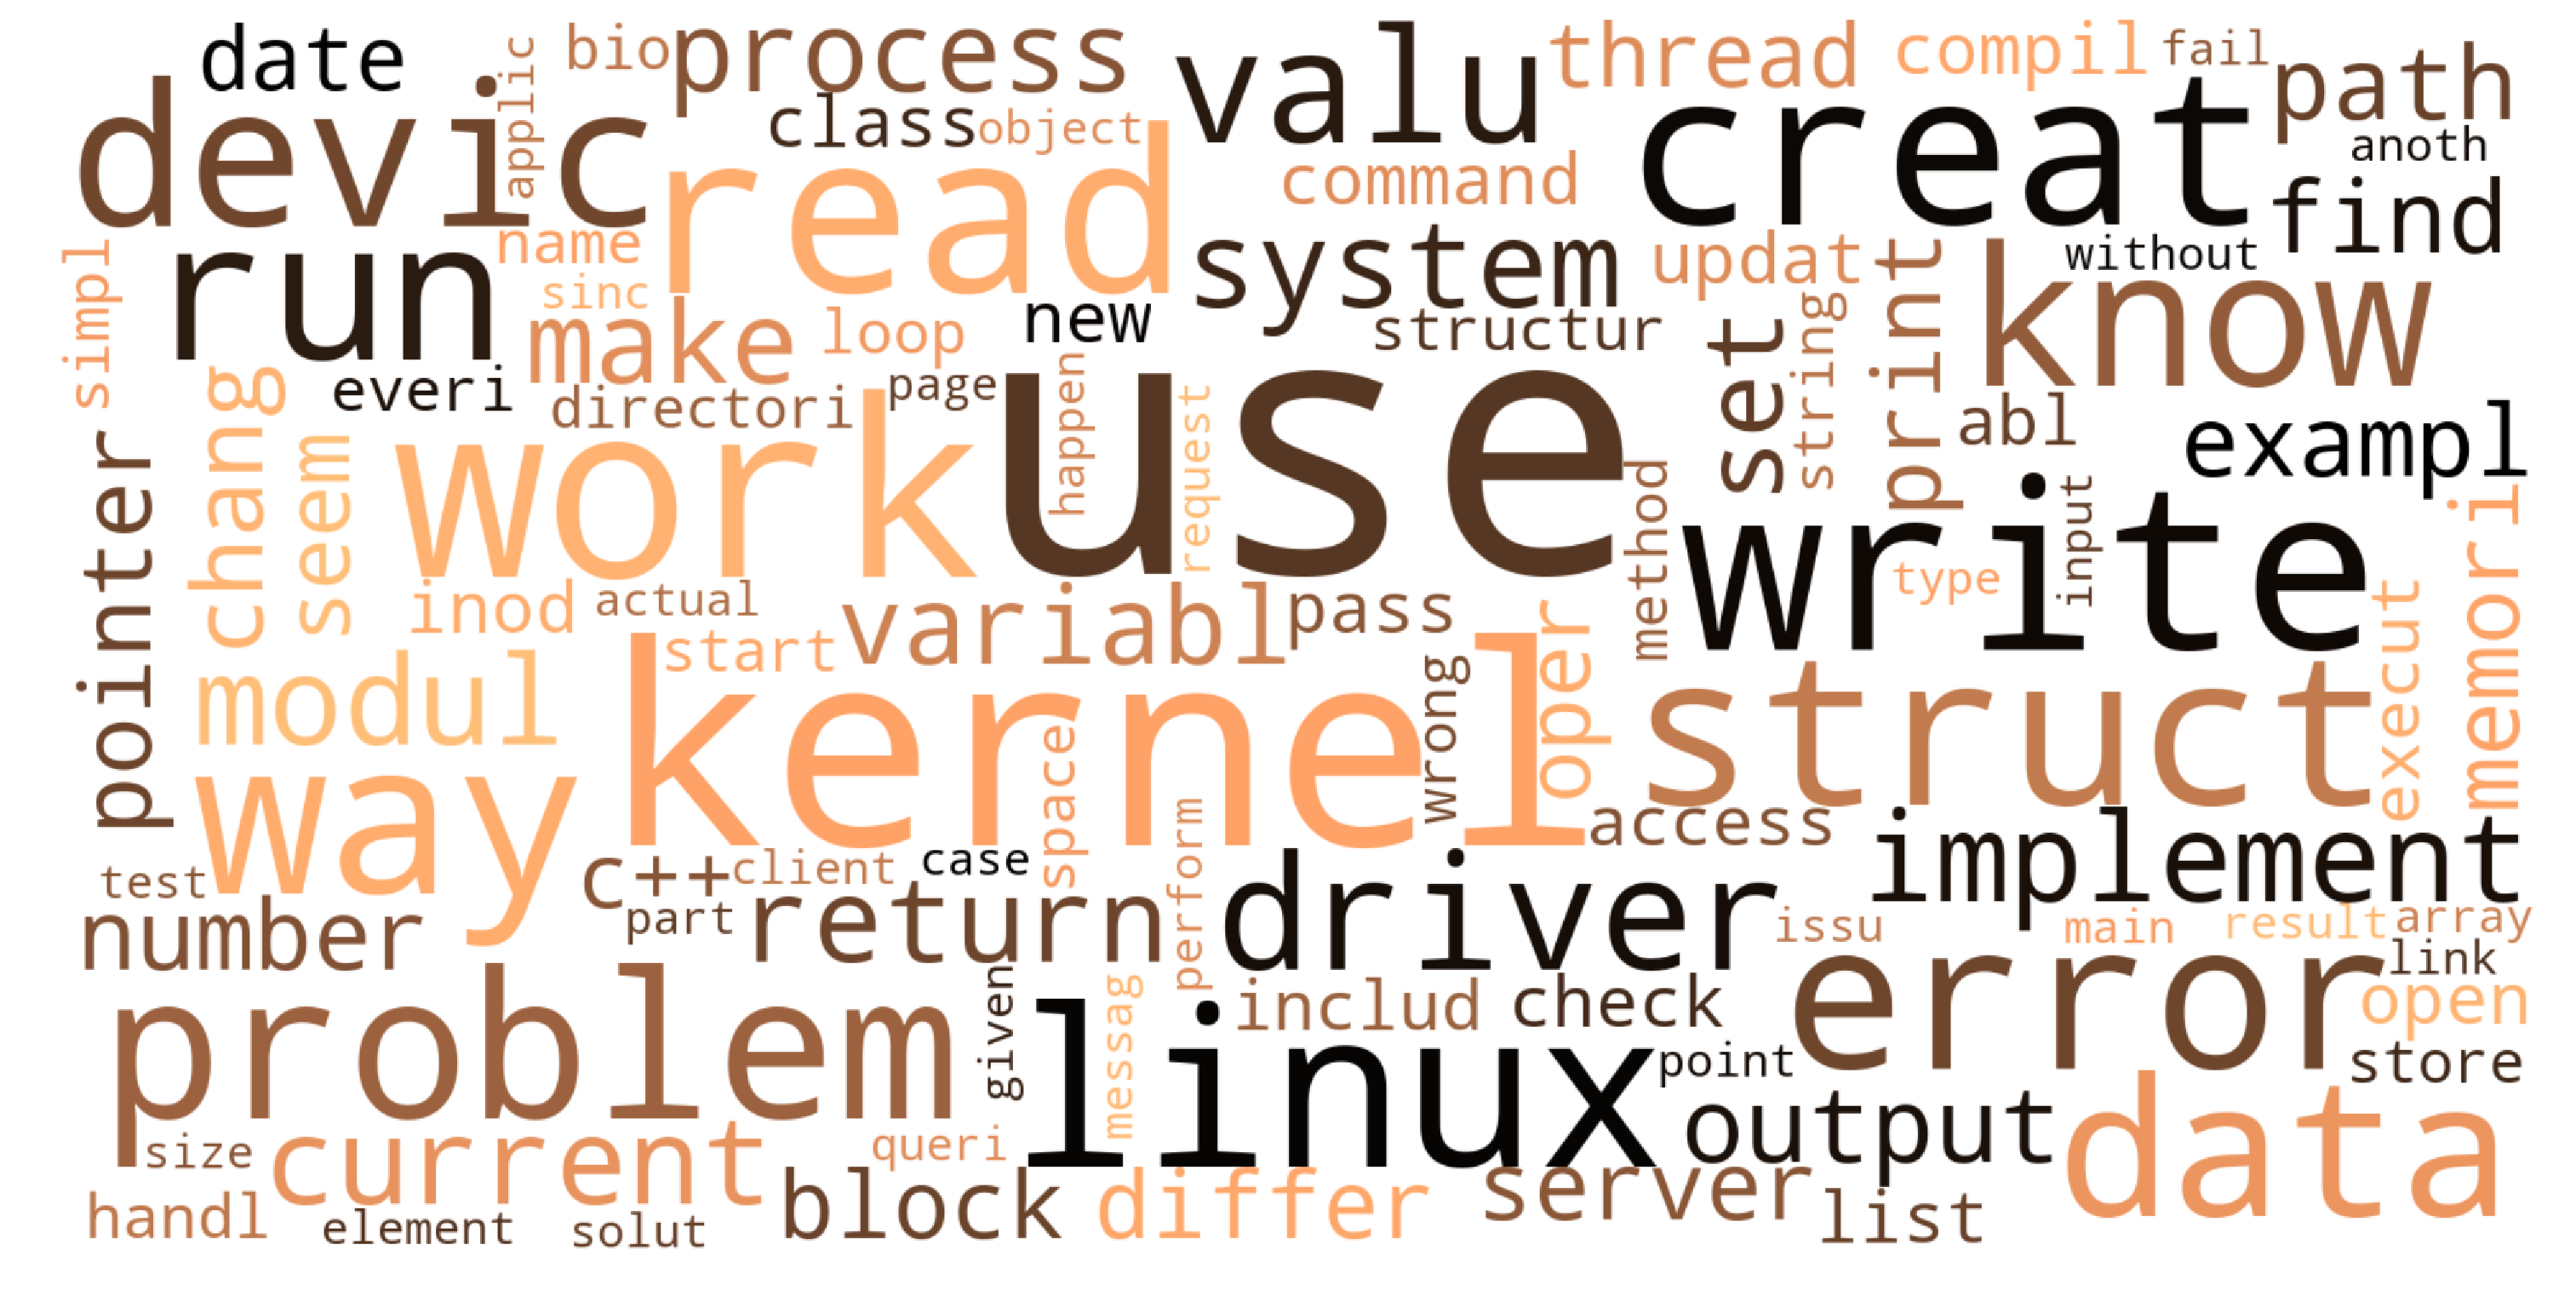
\includegraphics[width=\columnwidth]{scripts/figures/2-0-1-allquestions.pdf}}
  \subfloat[Bigrams]{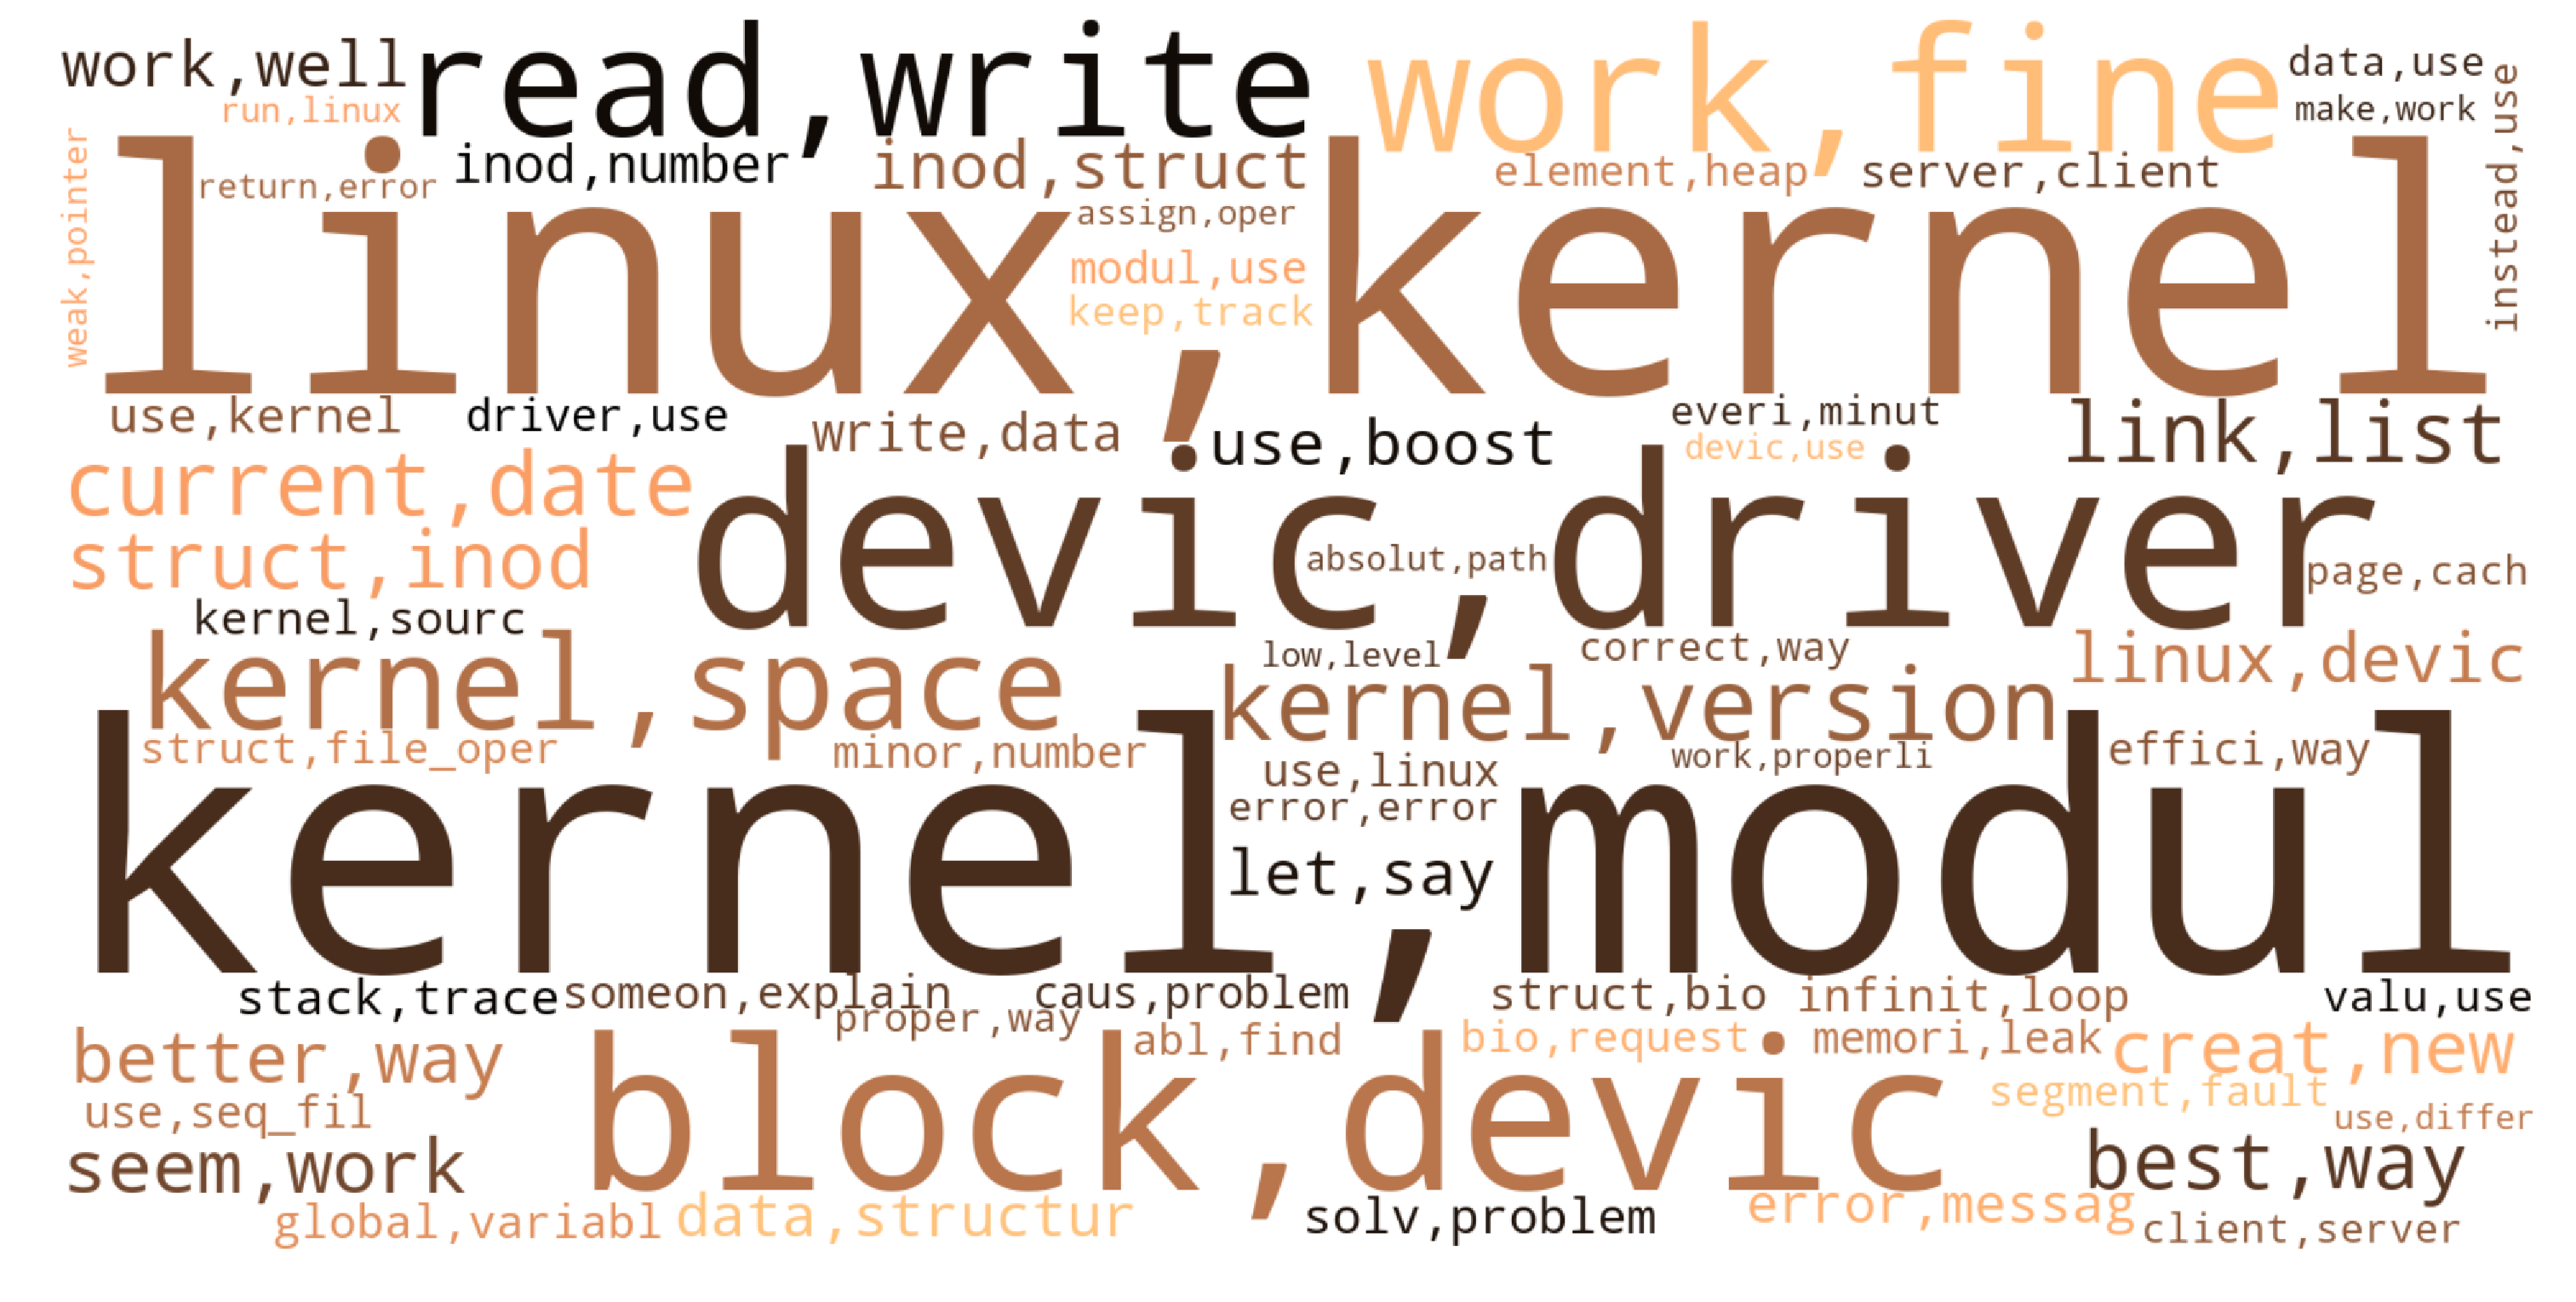
\includegraphics[width=\columnwidth]{scripts/figures/2-0-2-allquestions.pdf}}
  \caption{Word clouds generated by the most common words in all matching questions using single words (a) and bigrams (b)}
  \label{fig:wcall}
\end{figure*}

\subsubsection{Collocated Functions}
\textbf{RQ2.2 How often do pairs of components appear together in questions?}
This questions explores how often do questions ask about more than one function or API, giving insights about the codependence or confusion between functions. To achieve that, we search the recorded results from Subsection~\ref{subsec:analysis} for questions that contain two or more API functions. The Table~\ref{tab:samecat} shows the functions that appear together the most within the same category. From the results we can see that, within the same category, sequential file processing methods \texttt{seq\_*} are very commonly asked about together within the same question. This is because they are commonly used together to build device drivers, and many questions provide examples on how to use them, see this question\footnote{https://stackoverflow.com/q/17663692}, which discusses sequential file operations in device drivers.
Additionally, \texttt{debugfs\_create\_dir} and \texttt{debugfs\_create\_file} are commonly found together, since both of them can be used to create directories. The difference between them is that the former is the recommended function to create directories in debugfs, while the latter can be used to create directories and files alike. Most answers that reference both function explain this difference, including this one \footnote{https://stackoverflow.com/q/42235800}.
Debugfs\footnote{https://www.kernel.org/doc/Documentation/filesystems/debugfs.txt} is a simple-to-use RAM-based file system commonly used for debugging. For that reason, we can find many questions that contain examples for using different \texttt{debugfs\_*} functions at the same time.

\begin{table*}
  \caption{Top 10 functions that appear together from the same category}
  \label{tab:samecat}
  \begin{tabular}{cccc}
    \toprule
    Name & Name & Category & Occurrences \\
    \midrule
    \texttt{seq\_lseek} & \texttt{seq\_read} & Other VFS Functions & 41 \\
    \texttt{seq\_open}  & \texttt{seq\_read} & Other VFS Functions & 12 \\
    \texttt{seq\_lseek}  & \texttt{seq\_open} & Other VFS Functions & 11 \\
    \texttt{debugfs\_create\_dir} &  \texttt{debugfs\_create\_file} & The debugfs filesystem & 11 \\
    \texttt{seq\_lseek}  & \texttt{seq\_release} & Other VFS Functions & 10 \\
    \texttt{seq\_read}  & \texttt{seq\_release} & Other VFS Functions & 10 \\
    \texttt{seq\_open}  & \texttt{seq\_release} & Other VFS Functions & 9 \\
    \texttt{debugfs\_create\_file} & \texttt{debugfs\_remove} & The debugfs filesystem & 7 \\
    \texttt{debugfs\_create\_file} & \texttt{debugfs\_remove\_recursive} & The debugfs filesystem & 5 \\
    \texttt{debugfs\_create\_dir} & \texttt{debugfs\_remove\_recursive} & The debugfs filesystem & 4 \\
  \bottomrule
\end{tabular}
\end{table*}


summary

Threats to validity
Generalizability:  RQ1 generalizes findings of previus work in java api domain into the linux filesystem API domain, but it is still not known if this generalizes to other domains.
stackoverflow stuff
The remaining threats listed below arise from the fact that StackOverflow is unstructured
natural language text, and extracting information therefrom is naturally a noisy
process.
However, a mention of a class in an SO question or answer does not necessarily mean
that the message is about that class; but it does mean that the message is relevant somehow
to the class.
splitting
similar names
incorrect tags or formatting: often fixed by moderators.
Github only includes opensource projects in its search, which means that the usage data we derived is biased towards opensource projects. Github allows any user to fork any repository they want, this is mitigated by the github code search itself, since it does not include any forks that have less stars than the original repositories. there's a possibility of functions sharing the same name, but the function names we considered are unique enough as we concluded from manual inspection of the search results.
word frequency analysis might be biased towards functions that have more questions about them. This was not found to be a major concern in our analysis, but we could explore calculating the word frequency per function or category of functions.

future work
Qualitative study of the questions we found,
which can help produce machine learning models to predict stuff
Include other sources like linux mailing lists and issues in the study.
Expant to other linux kernel functions
We could use the


%TODO maybe search for other keywords with functions?













.
